\documentclass{rapport}
\usepackage{subcaption}
\usepackage{adjustbox}
\usepackage{lipsum}
\usepackage{gensymb}
\usepackage{float}
\usepackage{wrapfig}
\usepackage{amsmath} % Pour les environnements mathématiques
\usepackage{amssymb} % Pour les symboles supplémentaires comme R (réels)
\usepackage{graphicx} % Required for inserting images
\title{BE Automatique} %title of the file

\begin{document}

%----------- Report information ---------

\logo{logos/logo_n7.png}
\uni{\textbf{ENSEEIHT}}
\ttitle{Fonctionnalités - Projet long TOB\\Logiciel de montage vidéo} %title of the file
\subject{Fonctionnalités du logiciel de montage} % Subject name
\topic{Projet Long - TOB} % Topic name

\professor{G. \textsc{Dupont}} % information related to the professor

\students{Alexandre \textsc{Lescot}\\
          Camille \textsc{Meyer}\\
          Doryan \textsc{Benoit}\\
          Iman-Norr \textsc{Draou}\\
          Mathier \textsc{Trahand}\\
          Oscar \textsc{Mautin}\\
          Sophie \textsc{Girardot}\\
          Yacine  \textsc{Meziani}} % information related to the students

%----------- Init -------------------
        
\buildmargins % display margins
\buildcover % create the front cover of the document
\toc % creates the table of contents

%------------ Report body ----------------
\section{Objectif du projet}
Ce projet vise à développer une application de montage vidéo intuitive et performante, accessible aussi bien aux professionnels qu'aux débutants. L'objectif est de proposer un outil ergonomique permettant d'importer, d'éditer et de manipuler facilement du contenu multimédia.

\section{MVP}

\subsection{Timeline}
La timeline constitue la base du logiciel de montage. Il s'agit d'une frise chronologique sur laquelle les utilisateurs peuvent organiser leurs fichiers multimédias (vidéos, audios, images, textes). L’objectif est d’intégrer un système de \textit{drag and drop} permettant d’ajouter du contenu à la timeline et de le visualiser en temps réel dans la \textit{preview}.

Il sera également possible de manipuler les éléments sur la timeline : déplacer une vidéo de quelques secondes, assembler plusieurs fichiers ou ajuster leur durée. Les pistes vidéo (vidéos, images, textes) seront distinctes des pistes audio pour une meilleure gestion du contenu.

\subsection{Preview}
Un espace de prévisualisation sera intégré dans l’interface, permettant aux utilisateurs de visualiser les modifications effectuées sur la timeline en temps réel. La prévisualisation sera située dans la partie supérieure droite de la fenêtre, selon la conception définie.

\subsection{Importation de vidéos}
L’application offrira la possibilité d’importer des vidéos à partir du stockage local. Les utilisateurs pourront parcourir leurs documents et sélectionner un fichier à intégrer dans leur projet.

\subsection{Gestion des fichiers importés}
Une bibliothèque de médias affichera les fichiers importés, facilitant leur accès et leur organisation. Cet espace sera situé en haut à gauche de l’interface, conformément au design prévu.

\subsection{Ajout de vidéos à la timeline}
Les vidéos importées pourront être ajoutées à la timeline pour être manipulées. L’utilisateur pourra sélectionner un point précis de la vidéo à afficher en \textit{preview}, à l’aide d’un curseur dédié. D’autres actions de modification seront ajoutées ultérieurement.

\subsection{Lecture et manipulation des fichiers audio et vidéo}
Les fichiers vidéo et audio présents sur la timeline seront lisibles directement via la \textit{preview}, permettant un contrôle précis du montage.

\section{Fonctionnalités intermédiaires}

\subsection{Découpage de vidéos}
L’application permettra de découper une vidéo en plusieurs segments directement sur la timeline, à l’aide d’un curseur de sélection. Chaque segment pourra être déplacé indépendamment, supprimé ou réorganisé.

\subsection{Fusion de vidéos}
Les utilisateurs pourront assembler plusieurs vidéos pour en faire un seul fichier, facilitant le montage et l’édition de contenus combinés.

\subsection{Édition et lecture des fichiers audio}
Un fichier audio pourra être manipulé dans la timeline de la même manière qu’une vidéo. L’utilisateur pourra écouter un fichier, ajuster son placement et effectuer des modifications basiques.

\subsection{Ajout d’images à la timeline}
Les images pourront être intégrées dans la timeline et manipulées comme des vidéos, avec la possibilité de les visualiser dans la \textit{preview}.

\subsection{Exportation du montage}
L’application offrira une option d’export permettant de regrouper l’ensemble des éléments montés sur la timeline en un fichier final unique (ex. MP4). 

\section{Fonctionnalités supplémentaires}
\subsection{Ajout de texte à la timeline}
L’application permettra d’ajouter du texte personnalisable sur la timeline (possibilité de personnalisation de la police, la taille, la couleur, etc). L’utilisateur pourra définir la durée d’affichage du texte et le manipuler comme une vidéo ou une image. Ce texte pourra être positionné et édité.


\section{Croquis}
\begin{figure}[h]
    \centering
    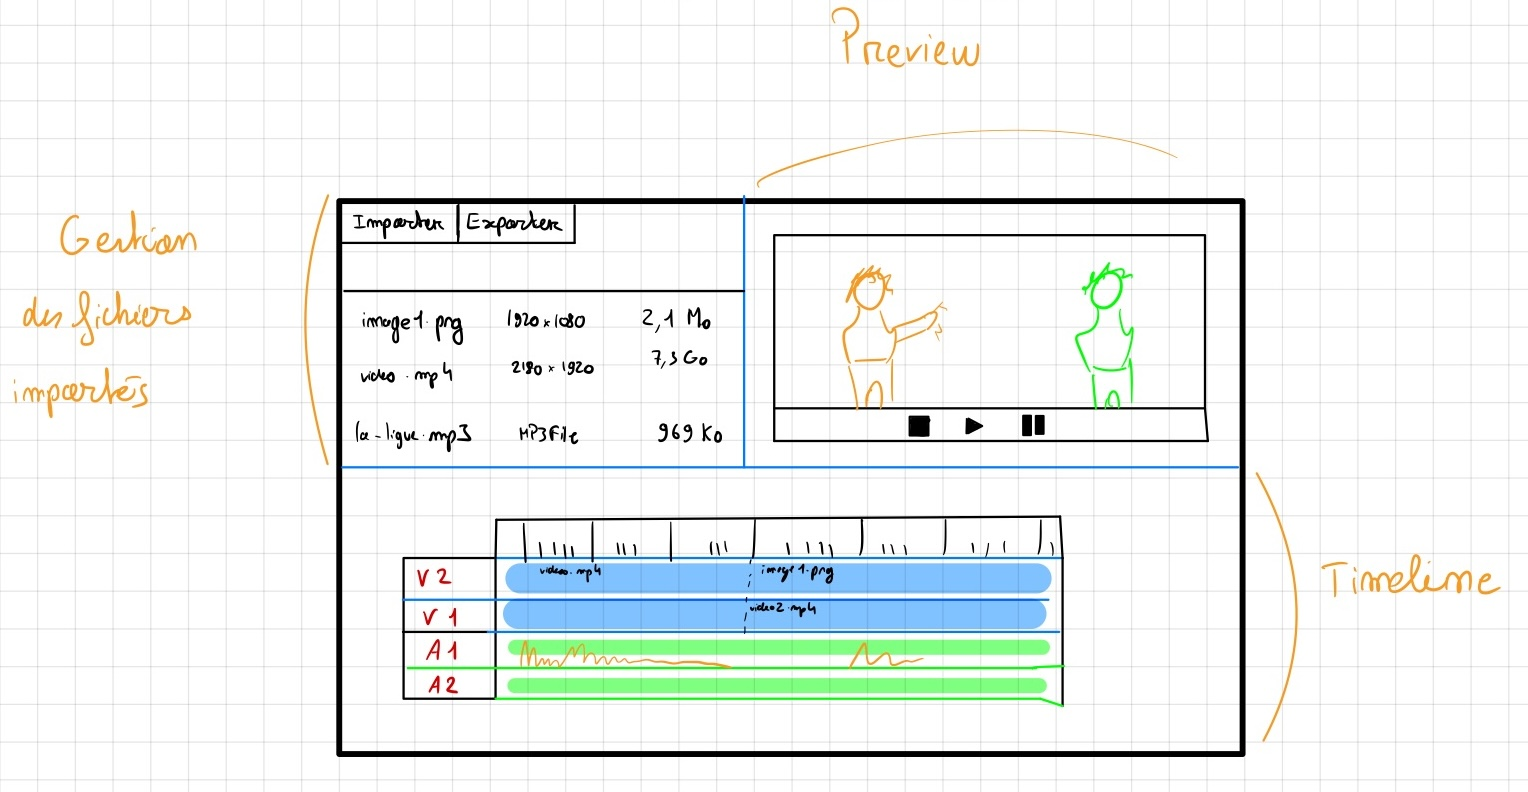
\includegraphics[width=1\textwidth]{croquis_v0.jpg}
    \caption{Premier croquis de l'application}
    \label{fig:croquis}
\end{figure}


\end{document}
